\begin{figure}[htb]
\begin{center}
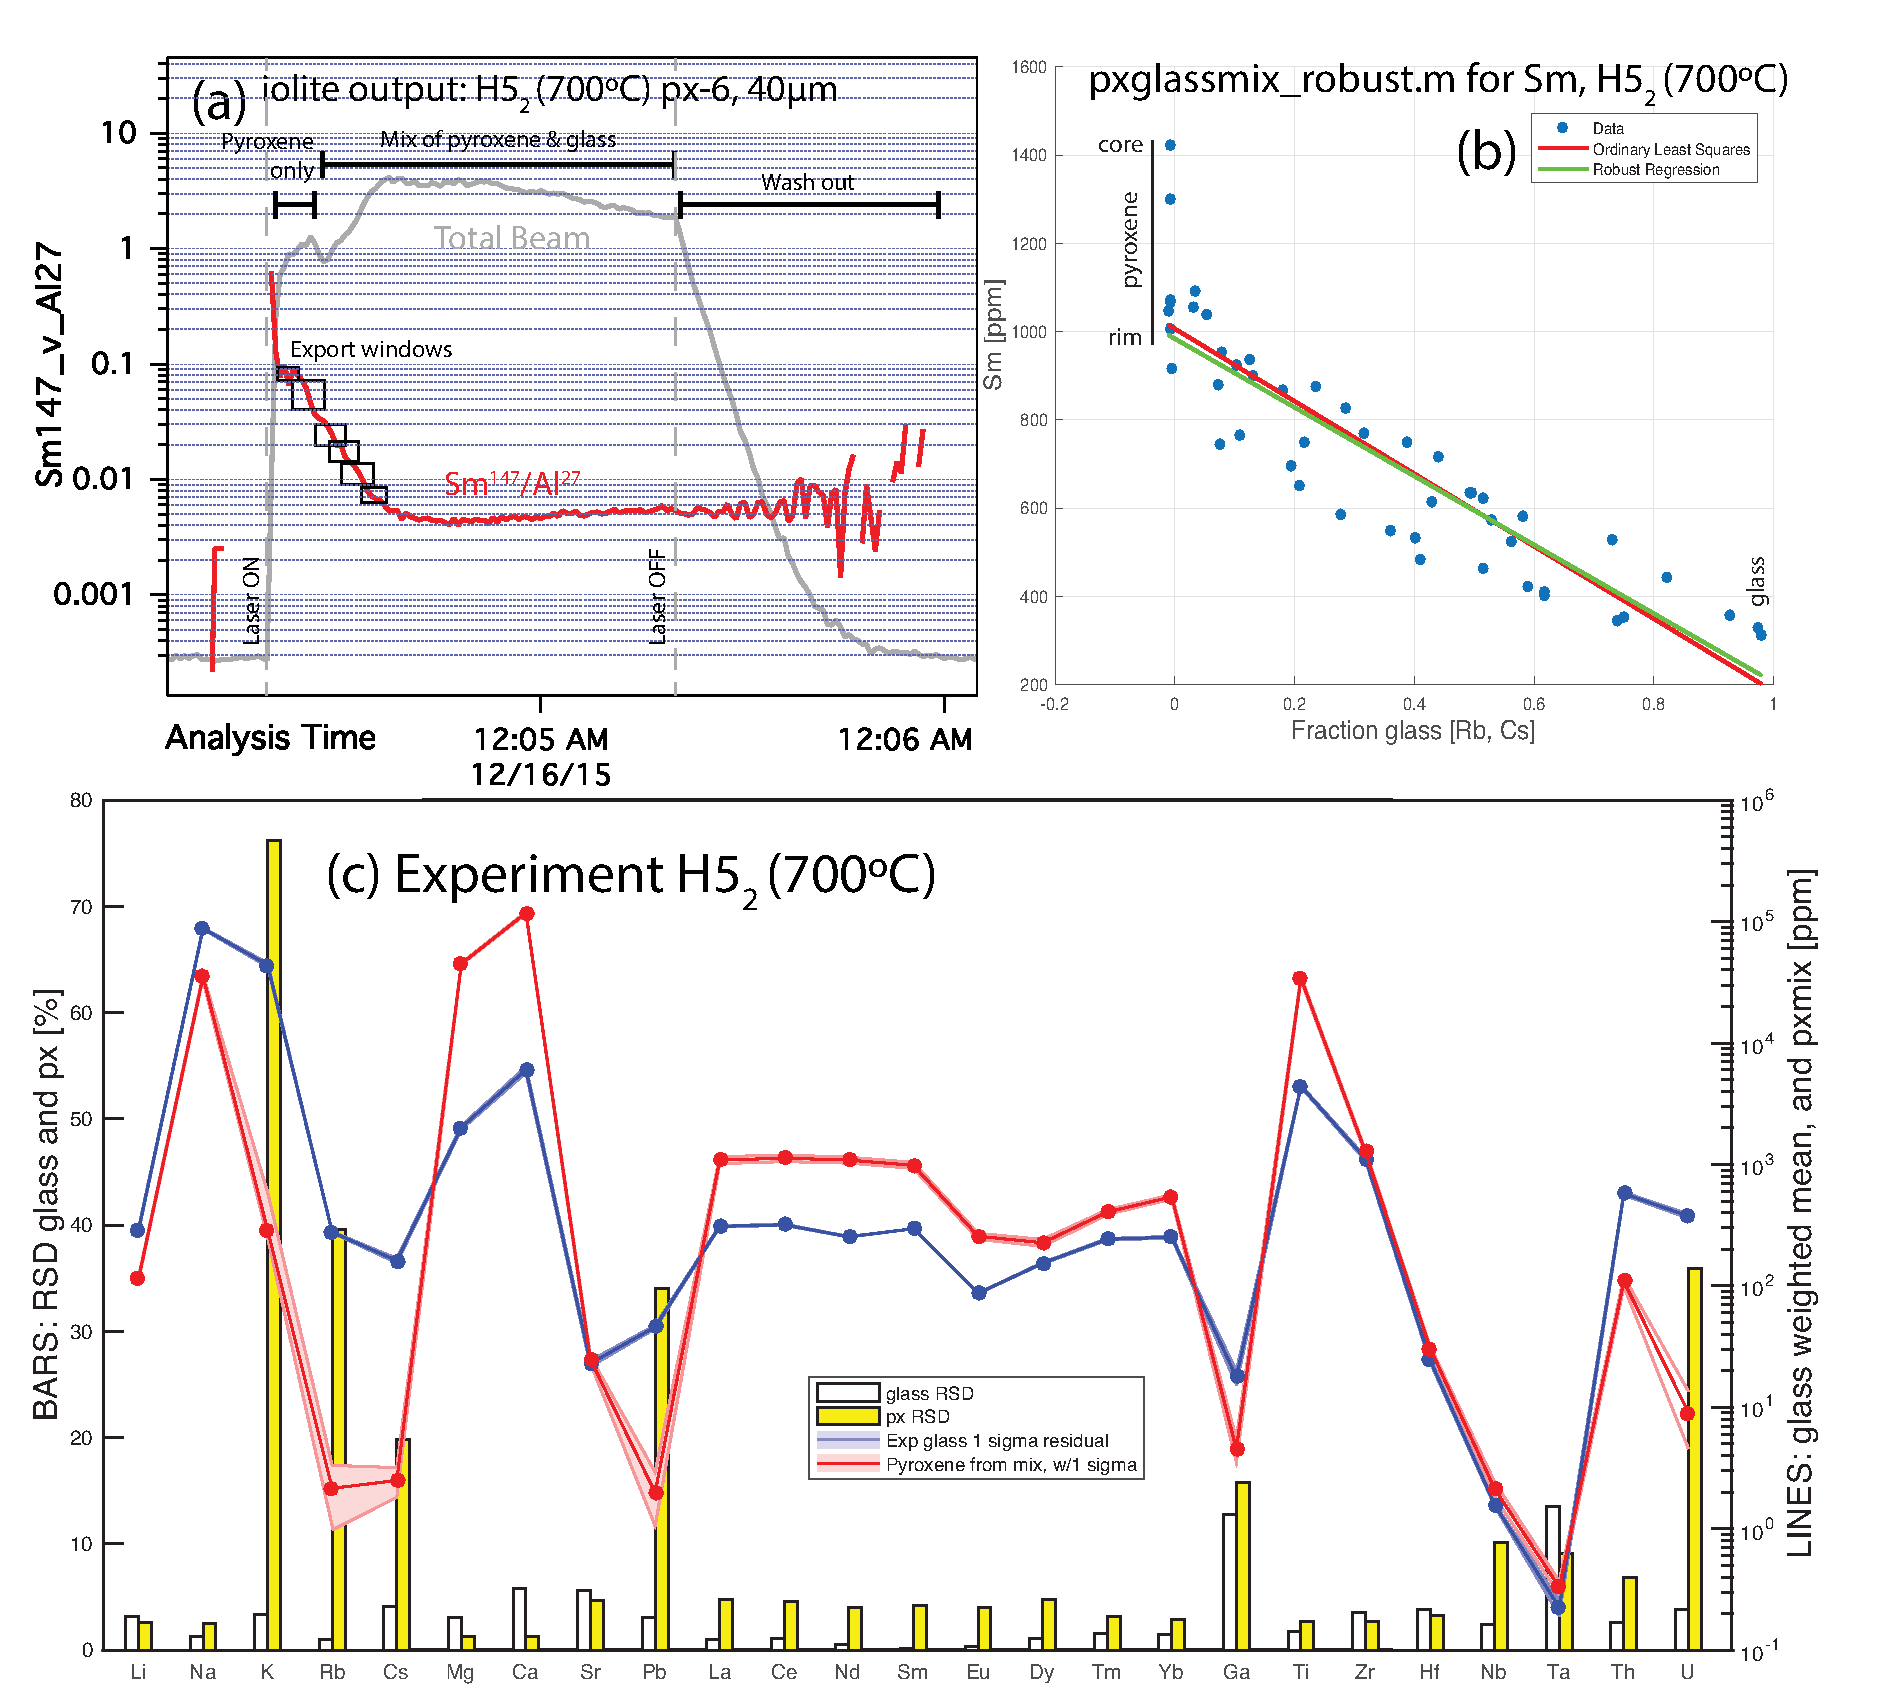
\includegraphics[width=0.85\textwidth]{S4_QAQC_LaserMix_H5_2}
\caption[An example of the robust regression data reduction scheme for laser-ablation ICP-MS analyses of glass and clinopyroxene mixtures.]
    {An example of the robust regression data reduction scheme for laser-ablation ICP-MS analyses of glass and clinopyroxene mixtures. (a) Time series of laser-ablation data as displayed in by the iolite v2.5 extension for Igor Pro \citep{Paton2011}, (b) a MATLAB output diagram from the robust regression unmixing script, and (c) a quality control diagram output from the same MATLAB script. %This data reduction methodology returns trace-element concentrations in clinopyroxene that are within analytical uncertainty of those derived via regular time-integrated data reduction methods.
    }
    \label{LaserMixFig}
\end{center}
\end{figure}

The LA-ICP-MS robust regression data reduction scheme described here allows for determination of mineral trace-element compositions where the grains of interest are smaller than the laser spot-size. The mathematics underpinning the script are similar those of \citet{Rubatto2007} and from our research group, of \citet{Yang2018}. 
Assumptions include...

		whilst effectively rejecting outlier data, for example from the ablation of minerals other than clinopyroxene that may have been hidden below the polished surfaces of the grain mounts




Initially, the raw counts-per-second data are imported into Igor Pro, running the iolite v2.5 extension \citep{Paton2011} where drift and background corrections are made. Mixed signals of clinopyroxene show characteristic stepped peaks in element-ratio and beam intensity traces (Figure \ref{LaserMixFig}a). Outputs are exported in short time windows as shown.

Trace-element concentrations in the mixes are then normalised to the sum of major-element oxides, as measured by LA-ICP-MS.

TO COMPLETE


(a) Time series of laser-ablation data, showing traces for Sm/Al (red) and total beam intensity (gray). The laser beam often ablated through the small clinopyroxene crystals, returning a mixed signal that was exported from the iolite data reduction software in short time windows as shown. Data were then normalised to the sum of major-element concentrations and mixes were deconvolved using a robust regression script written in MATLAB. (b) An example output diagram for the robust regression data reduction scheme. Clinopyroxene--glass mixing ratios were constrained by strongly incompatible elements Rb and Cs. For each element, a robust linear regression was defined between the fraction of glass in the mixture and element concentration. The intercept of this regression with zero glass returned the trace-element concentrations in the clinopyroxene. Uncertainty with this technique is typically below 10 \% relative (median 9.3 \% at the 1$\sigma$ level). In this example, the Sm-rich core of a zoned clinopyroxene crystal is effectively rejected during data processing, and the derived Sm concentration for the clinopyroxene is therefore closer to that of the clinopyroxene rims that are in equilibrium with the adjacent quenched melt. (c) A quality control diagram output from the MATLAB data reduction scheme showing the concentrations of various elements in the glass and clinopyroxene (lines) and the uncertainty on these concentrations expressed as a relative standard deviation (bars). Derived partition coefficients ($D_i$) are the mass concentration of element \emph{`i'} in clinopyroxene divided by that in the adjacent quenched melt. Residuals for the $D_i$ values were calculated using uncertainties derived from the clinopyroxene and glass analyses to calculate minimum and maximum partition coefficients at the 1$\sigma$ level. These are reported in Table \ref{D_table} and \ref{Ae_SupTbl}
